\section{ORBIT-SEED-R1: compact physical seeds and timestamp queries}
\label{sec:orbit}
This profile predicts the position of a satellite relative to a specified ground
station. It includes real MEO, GEO, inclined geosynchronous and high elliptical
examples. A small, complete model seed is the input; a requested timestamp is the
query. The model regenerates position and velocity with explicit dynamics. The
two ordered ASA/NA sets and the synchronous JK recurrence select subsequent
query times in ordered replay. Direct scrubbing obtains the same physical state
without replaying the preceding display interactions.

\begin{panel}
\textbf{Complete binary seeds; sizes are measured in the execution table.}\par
Each seed includes the initial state, force constants, compact Sun/Moon and frame
coefficients, provenance, both demonstration stations, time/query settings,
two ASA/NA mask sets and editable Boolean equations. No future target trajectory
table is stored. The native executable and its declared runtime are shared
dependencies, accounted for separately from per-seed bytes.
\end{panel}

The four fitted states use data at or before 2 January 2025 00:00 GPST. The
following seven days are excluded from fitting. Their earlier R1 results were
inspected before R2 development, so this interval is a reused benchmark.
These are archived examples,
not a statement of current satellite positions. An arbitrary future manoeuvre
cannot be recovered from a prior seed that does not contain that manoeuvre.
Compactness is a consequence of a specified dynamical model and initial
conditions; it does not provide lossless compression of every possible orbit.

\subsection{The complete state seed}
Let the decoded seed be
\begin{equation}
\mathcal S=(\mathcal I,t_0,\mathbf r_0,\mathbf v_0,\mathcal F,
\mathcal C,\mathcal M,\mathcal N,\mathcal G,\mathcal Q,\mathcal W,\mathcal P),
\end{equation}
where $\mathcal I$ identifies the object and model version, $\mathcal F$ contains
all force constants and fitted accelerations, $\mathcal C$ contains compact
planetary forcing, $\mathcal M$ defines the frame/time conversion,
$\mathcal N$ defines numerical integration, $\mathcal G$ defines the stations,
$\mathcal Q$ defines query/chart parameters, $\mathcal W$ defines the literal word
equations and masks, and $\mathcal P$ records construction provenance. Position
and velocity are six IEEE 754 binary64 SI numbers, not quantized UGTS addresses.

The upgraded physical model is \code{ORBIT-DYNAMICS-R2}; the decoder also retains
R1 support. Its state is geocentric and aligned
with GCRS/ICRF axes. Full GPST seconds since 6 January 1980 are retained. For an
elapsed query $\tau$, $t=t_0+\tau$ and
\begin{equation}
\mathrm{TT}=\mathrm{GPST}+51.184\ \mathrm{s},\qquad
\mathrm{JD}_{TT}=2444244.5+(t+51.184)/86400.
\end{equation}
The Chandra input is labelled TDB and is explicitly converted during construction
and review. GPST, UTC, TT and TDB calendar labels are not interchanged. At this
example epoch GPST is 18 seconds ahead of UTC.

\subsection{Explicit Earth frame and compact forcing}
Define the passive Earth rotation matrix and polar-motion matrix as
\begin{align}
R_z(a)&=\begin{pmatrix}\cos a&\sin a&0\\-\sin a&\cos a&0\\0&0&1\end{pmatrix},\\
P&=\begin{pmatrix}c_x&0&s_x\\s_y s_x&c_y&-s_y c_x\\-c_y s_x&s_y&c_y c_x\end{pmatrix},
\quad c_x=\cos x_p,\ s_x=\sin x_p,\ c_y=\cos y_p,\ s_y=\sin y_p.
\end{align}
With the embedded slowly varying celestial matrix $Q(\tau)$,
\begin{align}
a(\tau)&=a_0+\dot a\tau+\delta a(\tau),& M(\tau)&=P(\tau)R_z(a(\tau))Q(\tau),\\
\mathbf r_E&=M\mathbf r,& \mathbf v_E&=M\mathbf v+\dot M\mathbf r.
\end{align}
Thus Earth-fixed velocity includes the time derivative of the frame.
The construction uses IAU 2006/2000A and the IERS Bulletin A published on
26 December 2024, before the forecast epoch. Published daily $x_p,y_p$ and
DUT1 values are linearly interpolated. The ERA correction is
$\delta a(\tau)=\dot a[\mathrm{DUT1}(\tau)-\mathrm{DUT1}(0)]$, with
$\dot a=2\pi(1.00273781191135448)/86400$.
The velocity derivative includes $\dot P$, $\dot {\delta a}$ and $\dot Q$.
TIO locator $s'$ is zero. Published EOP predictions carry their own uncertainty;
their interpolation is not a future observed-EOP measurement.

Each slowly varying scalar coefficient block uses a finite Chebyshev expansion:
\begin{equation}
u(\tau)=\frac{2\tau-\tau_a-\tau_b}{\tau_b-\tau_a},\quad
f(\tau)=\sum_{k=0}^{d}c_k T_k(u),\quad
T_0=1,\ T_1=u,\ T_{k+1}=2uT_k-T_{k-1}.
\end{equation}
The seed stores the interval, degree and every coefficient. $Q$ has nine
degree-eighteen rows; Sun and Moon forcing have three rows of degree sixteen and
thirty respectively over the fifteen-day construction domain. Daily EOP blocks
have three degree-one rows: $\delta a,x_p,y_p$.
Rapid Earth rotation remains a direct trigonometric
rotation. At shared segment boundaries the later segment applies. Queries
outside the embedded domain return an error rather than silently extrapolating
the coefficient blocks.

The Sun/Moon coefficients approximate the DE440s planetary model published in
2020. They describe known forcing from other bodies, not withheld positions of
the target satellite. The measured off-node forcing discrepancies are about
1.99 m for the Sun and 0.060 m for the Moon. These quantities are not satellite
orbit accuracy. Original DE440 files are unnecessary during packed replay.

\subsection{Actual orbital differential equations}
The physical state evolves as
\begin{equation}
\frac{d\mathbf r}{d\tau}=\mathbf v,\qquad
\frac{d\mathbf v}{d\tau}=M^T\nabla_{\mathbf p}U(\mathbf p)
+\mathbf a_\odot+\mathbf a_{Moon}+\mathbf a_{SRP}+\mathbf a_{RTN}+\mathbf a_{GR},
\qquad \mathbf p=M\mathbf r.
\end{equation}
Here the Moon acceleration symbol denotes the declared lunar third-body term.
For $R=\|\mathbf p\|$, latitude sine $s=p_z/R$, longitude $\lambda$,
Earth radius $a_E$ and parameter $\mu$, the full degree/order twelve field is
\begin{equation}
U(\mathbf p)=\frac{\mu}{R}\sum_{n=0}^{12}\left(\frac{a_E}{R}\right)^n
\sum_{m=0}^{n}P_{nm}(s)[C_{nm}\cos(m\lambda)+S_{nm}\sin(m\lambda)].
\end{equation}
$P_{nm}$ has no Condon--Shortley phase. The seed stores unnormalized
$C_{nm},S_{nm}$, converted from the EGM96 fully normalized coefficients by
\begin{equation}
C_{nm}=\sqrt{(2-\delta_{m0})(2n+1)\frac{(n-m)!}{(n+m)!}}\,\overline C_{nm},
\end{equation}
and the same factor for $S$. It includes $C_{00}=1$ and $S_{00}=0$.
The positive-potential convention uses $+\nabla U$.

Native evaluation avoids longitude and polar division. Define
$X=a_Ep_x/R^2$, $Y=a_Ep_y/R^2$, $Z=a_Ep_z/R^2$, $D=a_E^2/R^2$,
$V_{00}=a_E/R$ and $W_{00}=0$. The Cartesian Cunningham recurrence is
\begin{align}
V_{mm}&=(2m-1)(XV_{m-1,m-1}-YW_{m-1,m-1}),\\
W_{mm}&=(2m-1)(XW_{m-1,m-1}+YV_{m-1,m-1}),\\
V_{nm}&=\frac{2n-1}{n-m}ZV_{n-1,m}
-\frac{n+m-1}{n-m}DV_{n-2,m},\\
W_{nm}&=\frac{2n-1}{n-m}ZW_{n-1,m}
-\frac{n+m-1}{n-m}DW_{n-2,m},\\
U&=\frac{\mu}{a_E}\sum_{n=0}^{12}\sum_{m=0}^{n}(C_{nm}V_{nm}+S_{nm}W_{nm}).
\end{align}
The diagonal recurrence uses $m=1,\ldots,12$; the off-diagonal recurrence uses
$m=0,\ldots,12$ and $n=m+1,\ldots,12$.
For $n=m+1$ the second term is absent. Each native recurrence value carries
three analytic Cartesian derivatives; the product rule produces $\nabla U$.
Independent Python validation differentiates the scalar potential with complex
steps, and native tests compare a separately coded spherical-gradient oracle.
The constants are $\mu=3.986004415\times10^{14}$ SI and $a_E=6378136.3$ m.
This is the tide-free EGM96 field truncated at degree/order twelve.

For each third body $b$ with Earth-centred position $\mathbf r_b$,
\begin{equation}
\mathbf a_b=\mu_b\left[
\frac{\mathbf r_b-\mathbf r}{\|\mathbf r_b-\mathbf r\|^3}
-\frac{\mathbf r_b}{\|\mathbf r_b\|^3}\right].
\end{equation}
The indirect term removes the acceleration of the Earth. With $\mathbf d=\mathbf
r-\mathbf r_\odot$, the fitted radiation-pressure term is
\begin{equation}
\mathbf a_{SRP}=\chi A\left(\frac{\mathrm{AU}}{\|\mathbf d\|}\right)^2
\frac{\mathbf d}{\|\mathbf d\|}.
\end{equation}
$\chi=0$ in the declared cylindrical Earth shadow when the seed's shadow flag is
enabled, and $1$ otherwise. With shadow disabled, $\chi=1$ everywhere. Explicitly,
if $\hat{\mathbf s}=\mathbf r_\odot/\|\mathbf r_\odot\|$, shadow requires
$\mathbf r\cdot\hat{\mathbf s}<0$ and
$\|\mathbf r-(\mathbf r\cdot\hat{\mathbf s})\hat{\mathbf s}\|<a_E$.
There is no hidden penumbra, attitude or manoeuvre model.
Finally,
\begin{align}
\hat{\mathbf R}&=\mathbf r/\|\mathbf r\|,&
\hat{\mathbf N}&=(\mathbf r\times\mathbf v)/\|\mathbf r\times\mathbf v\|,&
\hat{\mathbf T}&=\hat{\mathbf N}\times\hat{\mathbf R},\\
\mathbf a_{RTN}&=a_R\hat{\mathbf R}+a_T\hat{\mathbf T}+a_N\hat{\mathbf N}.
\end{align}
The Schwarzschild correction is explicit, with $r=\|\mathbf r\|$:
\begin{equation}
\mathbf a_{GR}=\frac{\mu}{c^2r^3}
\left[\left(\frac{4\mu}{r}-\mathbf v\cdot\mathbf v\right)\mathbf r
+4(\mathbf r\cdot\mathbf v)\mathbf v\right],\qquad c=299792458\ \mathrm{m/s}.
\end{equation}
The three signed empirical accelerations and $A$ are fitted only on the declared
training arc. Their continuation is a physical approximation, not knowledge of
future spacecraft operations. The same ten-parameter fit is fixed for all four
objects: state six, SRP one and RTN three. Earlier training-window candidates
of one, three and seven days are compared against the earlier January 1
interval; the lowest maximum error selects the window. The final fit uses
only data at or before the January 2 cutoff. This past-only selection is
distinct from the already inspected January 2--9 comparison benchmark.
Harmonics above degree twelve, tides, detailed radiation pressure, attitude
changes and manoeuvres remain possible sources of forecast disagreement.

\subsection{Bottom-up timestamp reconstruction and scrubbing}
Native CPU/CUDA integrate these equations with classical RK4. For a six-vector
$\mathbf y=(\mathbf r,\mathbf v)$ and derivative $F$,
\begin{align}
\mathbf k_1&=F(t,\mathbf y),&
\mathbf k_2&=F(t+h/2,\mathbf y+h\mathbf k_1/2),\\
\mathbf k_3&=F(t+h/2,\mathbf y+h\mathbf k_2/2),&
\mathbf k_4&=F(t+h,\mathbf y+h\mathbf k_3),\\
\mathbf y^+&=\mathbf y+\tfrac h6(\mathbf k_1+2\mathbf k_2+2\mathbf k_3+\mathbf k_4).
\end{align}
MEO/GEO/IGSO use $h=30$ seconds; Chandra uses $7.5$ seconds, selected through an
independent numerical-convergence check. Its fitted initial state and forces
were not refitted against future positions. Independent Python propagation uses
DOP853 rather than the native RK4 implementation.

For any elapsed time $\tau$, define $n=\operatorname{trunc}(\tau/h)$ and
$\epsilon=\tau-nh$. Canonical lattice states are obtained by repeated signed
steps from the packed epoch. The exact requested state is one final fractional
step of length $\epsilon$ from the canonical state at $nh$. Fractional results
never become canonical checkpoints. This makes the physical query independent
of the order in which the timeline was scrubbed.

The CPU worker retains at most the declared number of sparse checkpoints
(256 in the examples, at one-hour spacing). Missing checkpoints regenerate
from an available earlier canonical state or the epoch. Eviction changes work,
not the mathematical trajectory. Cold-query work is proportional to elapsed
integration steps; compact storage does not imply constant-time propagation.
CUDA batches assign independent timestamp queries to device work and integrate
from the epoch. They currently do not share the CPU checkpoint cache. CPU
scrubbing and parallel CUDA batch execution are distinct measured paths.

\subsection{Two vacuum/set stages and synchronous JK}
The user's ``double vacuum, double set'' is concretely defined here as exactly
two independently stored ASA/NA/boundary mask triples,
$(A_1,N_1,B_1)$ and $(A_2,N_2,B_2)$, applied in order. No unspecified operation is
inferred from the phrase. All operators below are 32-bit word operators, and
$P$ is the present mask. For stage $i$ and input $w$,
\begin{align}
a_i(w)&=w\mathbin\& A_i\mathbin\& P,\qquad
n_i(w)=a_i(w)\mathbin\&N_i,\\
h_i(w)&=\pop(n_i(w)\mathbin\&B_i),\qquad
V_i(w)=\begin{cases}0,&h_i(w)>0,\\n_i(w),&h_i(w)=0.\end{cases}
\end{align}
One selected boundary hit therefore absorbs the entire output word. It does
not merely clear the intersecting bit. At ordered query $j$,
\begin{align}
\mathbf s_j&=\Phi(\mathcal S,\tau_j),&
g_j&=G(\mathbf s_j,\mathcal G,\tau_j),\\
d_j&=E_D(g_j,\tau_j),&x_j&=E_X(q_j,d_j),\\
y_j&=V_2(V_1(x_j)),&J_j&=E_J(q_j,y_j,d_j),\\
K_j&=E_K(q_j,y_j,d_j),&
q_{j+1}&=[(J_j\mathbin\&\neg q_j)\mathbin| (\neg K_j\mathbin\&q_j)]\mathbin\&P,\\
\tau_{j+1}&=\min(\tau_{end},\tau_j+\Delta(q_{j+1})).
\end{align}
Both JK right-hand sides read the same old $q_j$. Boundary absorption does not
implicitly freeze JK. The editable X expression accepts $q,d$; J and K accept
$q,y,d$. They support word constants zero/ones and bitwise AND, OR, XOR and
complement with parentheses. They compile to literal
Boolean truth tables; an independent AST interpreter checks the complete trace.

Default predicate bits are, in ascending order: above the station elevation
mask, within three degrees of that mask, absolute seed age $|\tau|$ at least 24 hours, positive
elevation rate, and approaching range. The actual default expressions are
\begin{equation}
x=q\mathbin|d,\qquad J=y\mathbin\&d,\qquad K=\neg d.
\end{equation}
With both unabsorbed identity mask sets these reduce to $q^+=d$. The state still
selects the next physical query timestamp: $\Delta=30$ seconds when
$(q^+\mathbin\&6)\ne0$, and $300$ seconds otherwise. Different mask/equation
inputs change that recurrence, as the counterfactual and absorption tests
demonstrate. Physical acceleration never reads $q$; the CGK spring equations
are retained separately rather than renamed orbital gravity.

\subsection{Station-relative geometry and both horizons}
For WGS84 station position $\mathbf r_g$ and its standard East/North/Up rotation
$L(\varphi,\lambda)$,
\begin{equation}
\mathbf z=(E,N,U)^T=L(\mathbf r_E-\mathbf r_g),\qquad
\dot{\mathbf z}=L\mathbf v_E.
\end{equation}
Set $H=\sqrt{E^2+N^2}$ and $D=\|\mathbf z\|$. The returned quantities are
\begin{align}
\mathrm{az}&=\operatorname{atan2}(E,N)\bmod2\pi,&
\mathrm{el}&=\operatorname{atan2}(U,H),\\
\dot D&=\mathbf z\cdot\dot{\mathbf z}/D,&
\frac{d\sin\mathrm{el}}{dt}&=\dot U/D-U\dot D/D^2.
\end{align}
Azimuth is clockwise from North. At the horizontal origin azimuth and its
derivative are explicitly undefined. Angles are simultaneous geometric values:
there is no atmospheric refraction or retarded light-time correction here.

Visibility events solve
\begin{equation}
f(t)=\sin\mathrm{el}(t)-\sin\mathrm{el}_{mask}=0.
\end{equation}
The search refines sign brackets and derivative-bracketed extrema, so it can
recover a short pass whose sampled endpoints are both below the mask. It reports
grazing candidates and numerical root tolerances. The validation compares
120-second and 30-second searches over seven days for both stations and every
object. Without a global interval bound this is not a proof that arbitrarily
many roots cannot occur between samples. Always-visible/hidden labels mean
visible/hidden over the searched interval under the stated search policy.

The second horizon is an error-budget horizon. Given withheld reference samples
$\mathbf r^*_k$, $e_k=\|\mathbf r(t_k)-\mathbf r^*_k\|$. For budget $b$ the report
records the first sample with $e_k>b$ and its predecessor. The interval brackets
a sampled exceedance; it does not certify continuous error below $b$ before it.
An epoch can be inside the model's coefficient domain while outside a useful
accuracy horizon. Maximum error across the whole interval is reported alongside
endpoint error because an orbit can diverge and later approach the reference.

\subsection{Original UGTS keys and complete time}
The orbital chart uses $\rho=\log(H/r_0)$, $\theta=\operatorname{atan2}(N,E)$ and
the explicit separate hoop angle $\phi$. The source chart is used only when
$-20\le\rho\le0$; out-of-range coordinates are not wrapped into a valid key.
The full tick is $k=\lfloor t/\delta t\rfloor$, with integer winding and remainder
from $k=16384w+k_{phase}$. The normalized fraction is separately labelled
$k_{phase}/16384$. Source quantization produces the original
$(20,18,14,12)$-bit tuple. Both the contiguous and original Morton layouts are
retained. Full position, velocity, Up, absolute time and provenance remain in
the result. Source OTAN2 uses $\Delta\theta=\wrap(\theta_j-\theta_{j-1})$ and is
still $\arctan(\Delta\theta/\Delta\rho)$, with its
explicit undefined-ratio cases, and is not replaced by azimuth.

\subsection{Binary packing, integrity and executable entry points}
The 52-byte little-endian header contains magic \code{ATOMORB1}, format/codec
versions, compressed and raw lengths, and the SHA-256 of the domain-prefixed
canonical payload. The payload uses tagged null/Boolean/signed and unsigned
64-bit integer/binary64/string/list/map values. Map keys are sorted, unique UTF-8
strings. Codec 1 compresses those canonical bytes directly. The default codec 2
packs the numeric bit patterns into one-bit planes before Zlib compression.
It preserves all 64 bits per numeric value. For numeric word $w_j$, define
\begin{equation}
P_{b,g}=\sum_{\ell=0}^{63}
\left[\left(w_{64g+\ell}\mathbin{\mathrm{shr}}b\right)\mathbin\&1\right]2^\ell,
\quad b=0,\ldots,63.
\end{equation}
Absent final lanes are zero. The inverse restores bit $b$ of word $j$ from
lane $j\bmod64$ of $P_{b,\lfloor j/64\rfloor}$.
The plane-major uint64 words follow a structural template with original numeric
type tags, and a 16-byte \code{BITPLN64} header with template length and word count.
Signed integers, unsigned integers and binary64 preserve their original bits;
the structural template retains Boolean tokens. Both codecs share the same
canonical content digest. Plane packing adds zero numerical error, but does not
change floating-point arithmetic in propagation. The measured example packs are
slightly larger with this representation than with codec 1.
The decoder checks exact lengths,
bounded expansion and nesting, complete stream termination, canonical re-encoding,
digest, model schema and time domains. There is no executable payload or pickle.

The digest domain is \code{atomOS:ORBIT-SEED-R1:canonical-binary} followed by a
zero byte. Physical-model and complete-seed hashes differ by scope. Runtime
timings and cache occupancy are excluded from the deterministic trace digest;
all mathematical query fields and both mask/JK stages remain covered. Independent
verification reconstructs the native orbit, checks the full station geometry,
keys/time, OTAN2, the AST recurrence, next query time and final chain.

\begin{lstlisting}
python tools/orbital_seed.py inspect --seed examples/orbit/seeds/C03.orbseed
python tools/orbital_seed.py query --seed examples/orbit/seeds/C03.orbseed --worker bin/cpu/orbit_worker.exe --station singapore_demo --time-s 12345.678 --out NEW_QUERY.json
python tools/orbital_seed.py predict --seed examples/orbit/seeds/G05.orbseed --worker bin/cpu/orbit_worker.exe --end-s 86400 --out NEW_RUN
python tools/verify_orbit_run.py --seed examples/orbit/seeds/G05.orbseed --worker bin/cpu/orbit_worker.exe --run NEW_RUN --out NEW_VERIFY.json
python tools/orbit_scrub.py --worker bin/cpu/orbit_worker.exe
\end{lstlisting}
The local timeline is served at \url{http://127.0.0.1:3619}. It accepts exact
fractional-second queries, a slider, object/station selection, ordered feedback
playback and visibility events. The JSON companions are editable; packing them
rebuilds the binary \code{.orbseed} files with a new content identity. Accuracy reports are associated only when
their canonical physical-model hash matches the loaded seed.

\subsection{Packed execution and regression evidence}
The following numbers are derived from the final decoded seeds and verified
native binaries. The isolated replay child receives only the packed seed, shared
runtime source and native executable; an audit hook denies every read under the
original release directory. The reconstructed fractional, past and seven-day
timestamp states match the normal native run bit for bit.

\begin{center}\begin{tabular}{@{}lrrrr@{}}\toprule
Object & Seed bytes & Default queries & Altered JK & Warm max (ms)\\\midrule
G05 & 9,066 & 397 & 2,881 & 0.816\\
C03 & 9,074 & 289 & 2,881 & 0.956\\
C06 & 9,073 & 417 & 2,881 & 0.834\\
CHANDRA & 8,716 & 520 & 2,881 & 2.075\\
\bottomrule\end{tabular}\end{center}
Query counts cover one day. The counterfactual sets $J=1,K=0$ and changes the
actual timestamps selected by the native recurrence. Physical states at shared
timestamps remain identical. Warm timing is end-to-end Python/native geometry
latency on this host for the recorded fractional seek sequence, not a universal
performance bound. Cold seeks may require thousands of integration steps.

Across eight seven-day station/object searches, 83 rise/set events were found. The largest event-time change under refinement from 120-second to 30-second sampling was 0.002508 seconds. The event algorithm's grazing and no-global-root-exclusion qualifications still apply.


A five-minute, seven-day table containing time and six binary64 state components
would occupy 112,952 bytes before its metadata. This compares a generated state
table to its specified model, not arbitrary-trajectory compression.
The demonstration archive also contains
large reference datasets and audit traces, which are not per-seed replay inputs.

The table is 12.45 times the size of the largest complete packed seed. The shared CPU executable is 77,824 bytes, and the isolated shared Python source is 89,342 bytes at validation. Installed libraries and the OS/C++ runtime are additional shared dependencies. The default codec packs 64 one-bit planes into uint64 words without discarding any numeric bit. The canonical codec remains readable; bit-plane packing is slightly larger for these examples.

The new native orbital checks compare 1,040 CPU/CUDA positions across the four models, with maximum disagreement 0.00004320 m. All 256 complete CPU/CUDA two-stage word traces match. Bounded-cache stress tests remain bit-exact through repeated eviction. Compute Sanitizer reports zero errors for 129 orbital queries and the word operation. The full Python suite passes 139 tests, including bit-plane reconstruction, rehashed-false-geometry, OTAN2 rejection and missing-reference-interval acceptance.


Fresh retained-component regression passes four CTests on each build, 256 SATNAV
epochs per backend with independent reconstruction, 4,225 SRK transitions and
3,308 CGK transitions per backend, and 6,861 persistent live-worker comparisons
per backend. The required GPU review tool also records zero errors under both
texture and global-memory Compute Sanitizer runs on the actual RTX 5070 Ti Laptop.

The first orbital RK4 test exposed an omitted final state assignment; that defect
was fixed before these final results. Earlier failed and superseded investigation
folders are retained as such and are not used as final validation. Numerical
agreement is separate from the physical future-reference errors below.

% Evidence fragment: include in the orbital chapter. Retained booktabs,
% tabularx/Y, graphicx, hyperref and xurl suffice; no new packages.
\subsection{R2 physical-position results and separate confirmation}
\label{sec:orbit-validation}

The R2 models stay below the adopted \textbf{10 m three-dimensional
reference-discrepancy budget at every tested sample through 24 hours} for all
four targets, on both the January benchmark and the separate February
confirmation date. This statement concerns sampled positions of these seeds;
it is not a universal or continuous-time orbit guarantee.
The January window was previously inspected during R1 development and is
explicitly a \textbf{reused benchmark}. The February selection procedure was
frozen before its future errors were evaluated; no model was retuned afterward.

The forecast quantity is
\[
 e_i=\|\widehat{\boldsymbol r}(t_i)-\boldsymbol r_{\rm reference}(t_i)\|_2,
 \qquad t_i>t_0.
\]
The January origin is 2 January 2025 00:00 GPST,
$t_0=1419811200$; February uses 2 February 2025 00:00 GPST,
$t_0=1422489600$. All cutoff and earlier target rows are excluded from the
forecast curves. R2 selects among 1-, 3- and 7-day training windows using an
internal validation day entirely before the forecast origin. The selected
January windows are 3/3/3/1 days for G05/C03/C06/Chandra; the unchanged rule
selects 1/7/3/3 days for February. External EGM96 gravity and planetary forcing
are distinct from future target observations.

\begin{table}[htbp]
\centering\small
\caption{Maximum discrepancy over all first-day samples (metres). Each R2
column has 288 samples per target through 24 h; Chandra's final sample is
approximately 51.185 s before the exact endpoint.}
\label{tab:orbit-first-day-comparison}
\begin{tabular*}{\linewidth}{@{\extracolsep{\fill}}lrrr@{}}
\toprule
Target & R1 January & R2 January & R2 February\\
\midrule
G05 / MEO & 285.330 & 1.057 & 3.072\\
C03 / GEO & 20.600 & 5.304 & 4.654\\
C06 / IGSO & 44.684 & 1.172 & 2.108\\
Chandra / HEO & 76.506 & 8.093 & 0.290\\
\bottomrule
\end{tabular*}
\end{table}

\begin{table}[htbp]
\centering\small
\caption{R2 January discrepancy in metres at the nearest actual sample to each
requested horizon. Individual samples are not worst-case interval errors.}
\label{tab:orbit-horizon-samples}
\begin{tabular*}{\linewidth}{@{\extracolsep{\fill}}lrrrrrr@{}}
\toprule
Target & 15 min & 1 h & 6 h & 24 h & 72 h & 7 d\\
\midrule
G05 / MEO & 0.474 & 0.655 & 0.272 & 0.713 & 2.228 & 12.531\\
C03 / GEO & 1.368 & 1.702 & 4.350 & 4.172 & 17.939 & 73.481\\
C06 / IGSO & 0.547 & 0.609 & 0.615 & 1.172 & 2.335 & 2.360\\
Chandra / HEO & 0.003 & 0.008 & 0.074 & 2.052 & 28.338 & 3680.247\\
\bottomrule
\end{tabular*}
\end{table}

\textbf{Time grid.} GNSS is on the exact requested GPST grid. Chandra is supplied
on a 300 s TDB grid, converted using the periodic TDB--TT correction and
$\mathrm{GPST}=\mathrm{TT}-51.184\,\mathrm{s}$. The nearest 15 min sample is
848.816057 s after the January origin and 848.815204 s after the February
origin. The final samples are respectively 604748.815856 s and
604748.815036 s. Exact offsets remain in the CSV/JSON, including all six
requested horizons for both dates.

\begin{table}[htbp]
\centering\small
\caption{R2 whole-window statistics (metres). January has 2,016 samples per
target. February has 2,016 each except C03, which has 1,441 and a 48 h gap.}
\label{tab:orbit-period-errors}
\begin{tabular*}{\linewidth}{@{\extracolsep{\fill}}lrrrr@{}}
\toprule
Target & Jan. RMS & Jan. maximum & Feb. RMS & Feb. maximum\\
\midrule
G05 / MEO & 5.294 & 12.998 & 33.113 & 71.800\\
C03 / GEO & 37.434 & 78.717 & 39382.862 & 100604.174\\
C06 / IGSO & 2.943 & 8.084 & 3.494 & 7.629\\
Chandra / HEO & 5412.235 & 25635.951 & 2055.685 & 5663.182\\
\bottomrule
\end{tabular*}
\end{table}

The seven-day 10 m budget is \textbf{not met for all targets}. C06 stays
below it at every seven-day sample on both dates; G05 exceeds it later on both
dates. C03 and Chandra have additional reference qualifications below.
The original R1 seven-day maxima were 7402.960/532.582/1237.242/19399.307 m
in the same object order. The R2 first-day improvement must not be extended
into a claim that every seven-day maximum improved or passed.
RMS and percentiles describe correlated samples, not independent-sample
confidence intervals. Reports additionally retain interval RMS/maxima and
sample percentiles.

\subsection{Sampled thresholds and incomplete reference coverage}
\label{sec:orbit-thresholds}
\begin{table}[htbp]
\centering\small
\caption{Preceding sample and first sampled exceedance, in hours after the
origin, rounded to 0.001 h. These pairs are not certified continuous crossing
brackets. ``None'' means no exceedance at the available samples.}
\label{tab:orbit-first-exceedance}
\begin{tabularx}{\linewidth}{@{}llYYY@{}}
\toprule
Date & Target & 10 m & 100 m & 1 km\\
\midrule
January & G05 / MEO & $(145.083,145.167]$ & None at samples & None at samples\\
January & C03 / GEO & $(29.000,29.083]$ & None at samples & None at samples\\
January & C06 / IGSO & None at samples & None at samples & None at samples\\
January & Chandra / HEO & $(50.402,50.486]$ & $(82.569,82.652]$ & $(83.986,84.069]$\\
February & G05 / MEO & $(50.833,50.917]$ & None at samples & None at samples\\
February & C03 / GEO & $(72.000,120.000]$ & $(72.000,120.000]$ & $(72.000,120.000]$\\
February & C06 / IGSO & None at samples & None at samples & None at samples\\
February & Chandra / HEO & $(83.986,84.069]$ & $(83.986,84.069]$ & $(83.986,84.069]$\\
\bottomrule
\end{tabularx}
\end{table}

For 10 km, January Chandra first exceeds the level at 302648.815956 s,
following the sample at 302348.815956 s; all January GNSS targets remain below
10 km at their samples. February C03 first exceeds 10 km at the first sample
after its gap, 432000 s; the previous sample is at 259200 s. Other February
targets remain below 10 km at the sampled times.

\textbf{C03 February coverage.} GFZ contains no C03 records on February 5 and
6. Adjacent daily endpoints leave a 48-hour reference gap and 575 missing
five-minute samples. Wuhan also lacks C03 on February 6 and cannot certify the
missing interval. GFZ remains the predeclared primary source. The first
post-gap discrepancy is 29256.547 m and the later maximum is 100604.174 m;
these observed exceedances are retained. Full-window coverage is
\textbf{indeterminate}, and no continuous tolerance passage through the gap is
inferred. No maneuver or other cause is assigned from missing records alone.
The figures leave the missing interval blank.

\subsection{Numerical error and reference discontinuities}
\label{sec:orbit-error-separation}
\begin{table}[htbp]
\centering\small
\caption{Separate numerical and frame comparisons, in metres. January's
independent physical audit uses 11 times across the past/future domain;
February compares nine future checkpoints with adaptive DOP853. The frame
column is the larger of the two complete sampled frame-approximation maxima.}
\label{tab:orbit-error-components}
\begin{tabular*}{\linewidth}{@{\extracolsep{\fill}}lrrr@{}}
\toprule
Target & Jan. RK4/DOP853 & Feb. RK4/DOP853 & Frame approximation\\
\midrule
G05 / MEO & 0.031716 & 0.026461 & 0.002007\\
C03 / GEO & 0.001232 & 0.001023 & 0.003260\\
C06 / IGSO & 0.001252 & 0.001026 & 0.003169\\
Chandra / HEO & 0.036582 & 0.147044 & 0.009135\\
\bottomrule
\end{tabular*}
\end{table}

Native RK4 uses 30 s for GNSS and 7.5 s for Chandra. Same-seed integration
agreement tests arithmetic, not orbit truth. The January forecast report's
own DOP853 check covers only its first sample; the wider January evidence above
comes from the separate, target-independent physical audit. Native CPU/CUDA
checks and exact word/packing checks remain separate evidence.
The frame test compares the embedded daily-EOP/Chebyshev frame with direct SOFA
IAU 2006/2000A evaluation of the same published prediction. It excludes actual
future EOP error, station uncertainty and a complete relativistic ICRF/GCRS
coordinate error budget; it is not subtracted as an independent scalar variance.

\begingroup\clubpenalty=10000
\textbf{Chandra source discontinuities.} The January error rises from
123.204 m to 23839.033 m between two five-minute samples. A separate one-second
Horizons query shows that at January 5 TDB 12:01:09--12:01:10 the source
position displacement differs from the integral of its own reported velocity
by \textbf{24317.077 m}; outside the neighboring jump intervals the same local
check is at most 0.0654 m. Native RK4 agrees with independently tightened
DOP853 to about 1.5 mm at the two forecast endpoints surrounding that jump.
The source header identifies CFA's merged trajectory, but no local join or
maneuver cause. The large discontinuity therefore cannot be attributed solely
to smooth force error or native integration.
\par\endgroup

The February reference has a corresponding kinematic discontinuity at
February 5 TDB 12:01:09--12:01:10: \textbf{2487.123 m} displacement-minus-velocity
integral mismatch, versus at most $2.26\,\mu\mathrm{m}$ away from its neighboring
intervals. The forecast's next five-minute error rises from 1.053 m to
2492.098 m. These diagnostics use only the source's positions and velocities;
no model is fitted to them. \textbf{All original discrepancy samples and
whole-window maxima are retained.} The cause of the provider discontinuities
is not established, and no corrected ``true orbit'' accuracy is invented.
Original queries, hashes and calculations are in
\path{source/orbit_data/diagnostics/}.

\textbf{Reference uncertainty.} January GFZ/Wuhan comparisons give 3D RMS
0.0263 m for G05, 2.074 m for C03 and 0.1692 m for C06; C03's maximum provider
disagreement is 3.575 m. These are product differences, not certified absolute
bounds. Providers share some underlying observations. Chandra supplies no
state covariance or absolute position guarantee. A millimetre or sub-metre
match to a selected reference is therefore not a matching physical-accuracy
claim.

\subsection{Chronology, source conventions and reproducible evidence}
\label{sec:orbit-provenance}
The R2 physical model uses the documented degree/order-12 EGM96 field,
cutoff-available daily Earth orientation, and external Sun/Moon forcing.
EGM96's original mu, reference radius, tide-free convention and fully normalized
coefficients are preserved with explicit conversion in
\path{source/orbit_data/gravity_reference/}. The format's normalization default
is documented by ICGEM:
\url{https://icgem.gfz.de/docs/ICGEM-Format-2023.pdf}.

The EOP sources were published before their cutoffs: IERS Bulletin A of
26 December 2024 and 30 January 2025, respectively:
\url{https://datacenter.iers.org/data/6/bulletina-xxxvii-052.txt} and
\url{https://datacenter.iers.org/data/6/bulletina-xxxviii-005.txt}.
Both permit public release and unlimited distribution.
The February GFZ reference changes from IGS20 to IGb20. IGSMAIL-8543, published
9 December 2024, specifies zero datum transformation parameters because origin,
scale and orientation remain aligned; individual reference-station coordinates
are updated. Preserve each source label and apply no fitted alignment:
\url{https://lists.igs.org/pipermail/igsmail/2024/008539.html}.

Precise target products were retrieved retrospectively; their earlier estimates
can incorporate later observations within provider processing. Neither date
proves that identical seeds were available live in 2025. January is a reused
comparison, while February applies the already-frozen selection rule to a
separate date. The confirmation freeze manifest binds the rule and model-file
hashes. Raw source acquisition and coverage inspection preceded any February
prediction-error evaluation. No later error was used to refit a seed.

\begin{itemize}
\item \textbf{GFZ and IGS.} Retain GFZ/IGS provider and network attribution.
The cited GFZ product-series DOI is
\url{https://doi.org/10.5880/GFZ.1.1.2016.003}; its DataCite record declares
\textbf{CC BY-NC 4.0}. The DOI names an ultra-rapid series whereas these GBM
files are rapid products without a separate per-file grant. The fixture bundle
conservatively retains that noncommercial qualification and is not claimed as
unrestricted commercial data. IGS terms:
\url{https://www.igs.org/wp-content/uploads/2020/09/IGS-Data-and-Product-Disclaimer-and-Terms-of-Use-200805.pdf}.
\item \begin{minipage}[t]{\linewidth}\textbf{CODE and Wuhan.} CODE's reference
\url{https://doi.org/10.48350/197028} lists open access/BORIS terms, not a blanket
MIT grant. Wuhan final products retain provider/IGS attribution. Original
archive URLs and per-file hashes remain in the source manifests.\end{minipage}
\item \textbf{NASA/JPL and CFA.} Acknowledge Giorgini and the JPL Solar System
Dynamics Group, NASA/JPL Horizons, and CFA for Chandra:
\url{https://ssd.jpl.nasa.gov/horizons/}.
Retrieval date is 15 September 2026. Geometric ICRF/TDB settings and original
responses are retained. Sun/Moon Horizons responses identify DE441; the
construction oracle is DE440s, a distinct planetary ephemeris version.
\end{itemize}

\textbf{Authoritative reports.} Use
\path{results/orbit_accuracy_r2_cpu_verified/accuracy_summary.json}, its CUDA
counterpart, and
\path{results/orbit_accuracy_confirmation_cpu_verified/accuracy_summary.json}.
R1 evidence remains in \path{results/orbit_accuracy_cpu_final/} for comparison.
The pre-fix failed trial and superseded intermediate models are not final
accuracy evidence. CSVs retain every measured error, exact horizon offset,
source and frame. Each report distinguishes \path{model_file_sha256} from
\path{physical_model_sha256}=\path{orbit_seed.digest(model)}; legacy
\path{model_sha256} is explicitly the file-hash alias. Accuracy displayed for a
custom packed seed applies only when the physical-model digest matches.
Reference fixtures, publications and the DE440s construction binary are
separate from the complete replay seed byte count.

\clearpage
\subsection{R2 January benchmark curves}
\label{sec:orbit-first-day-plot}
\begin{center}

\includegraphics[width=\linewidth]{../results/orbit_accuracy_r2_cpu_verified/forecast_error_curves.pdf}
\end{center}
This is the reused January benchmark. Dotted lines are reporting thresholds,
not fitted constraints. The Chandra source discontinuity remains visible and
its errors remain counted. First-day detail is also supplied as
\path{forecast_error_first_day.pdf} in the same result directory.

\clearpage
\subsection{Separate February confirmation curves}
\label{sec:orbit-full-week-plot}
\begin{center}
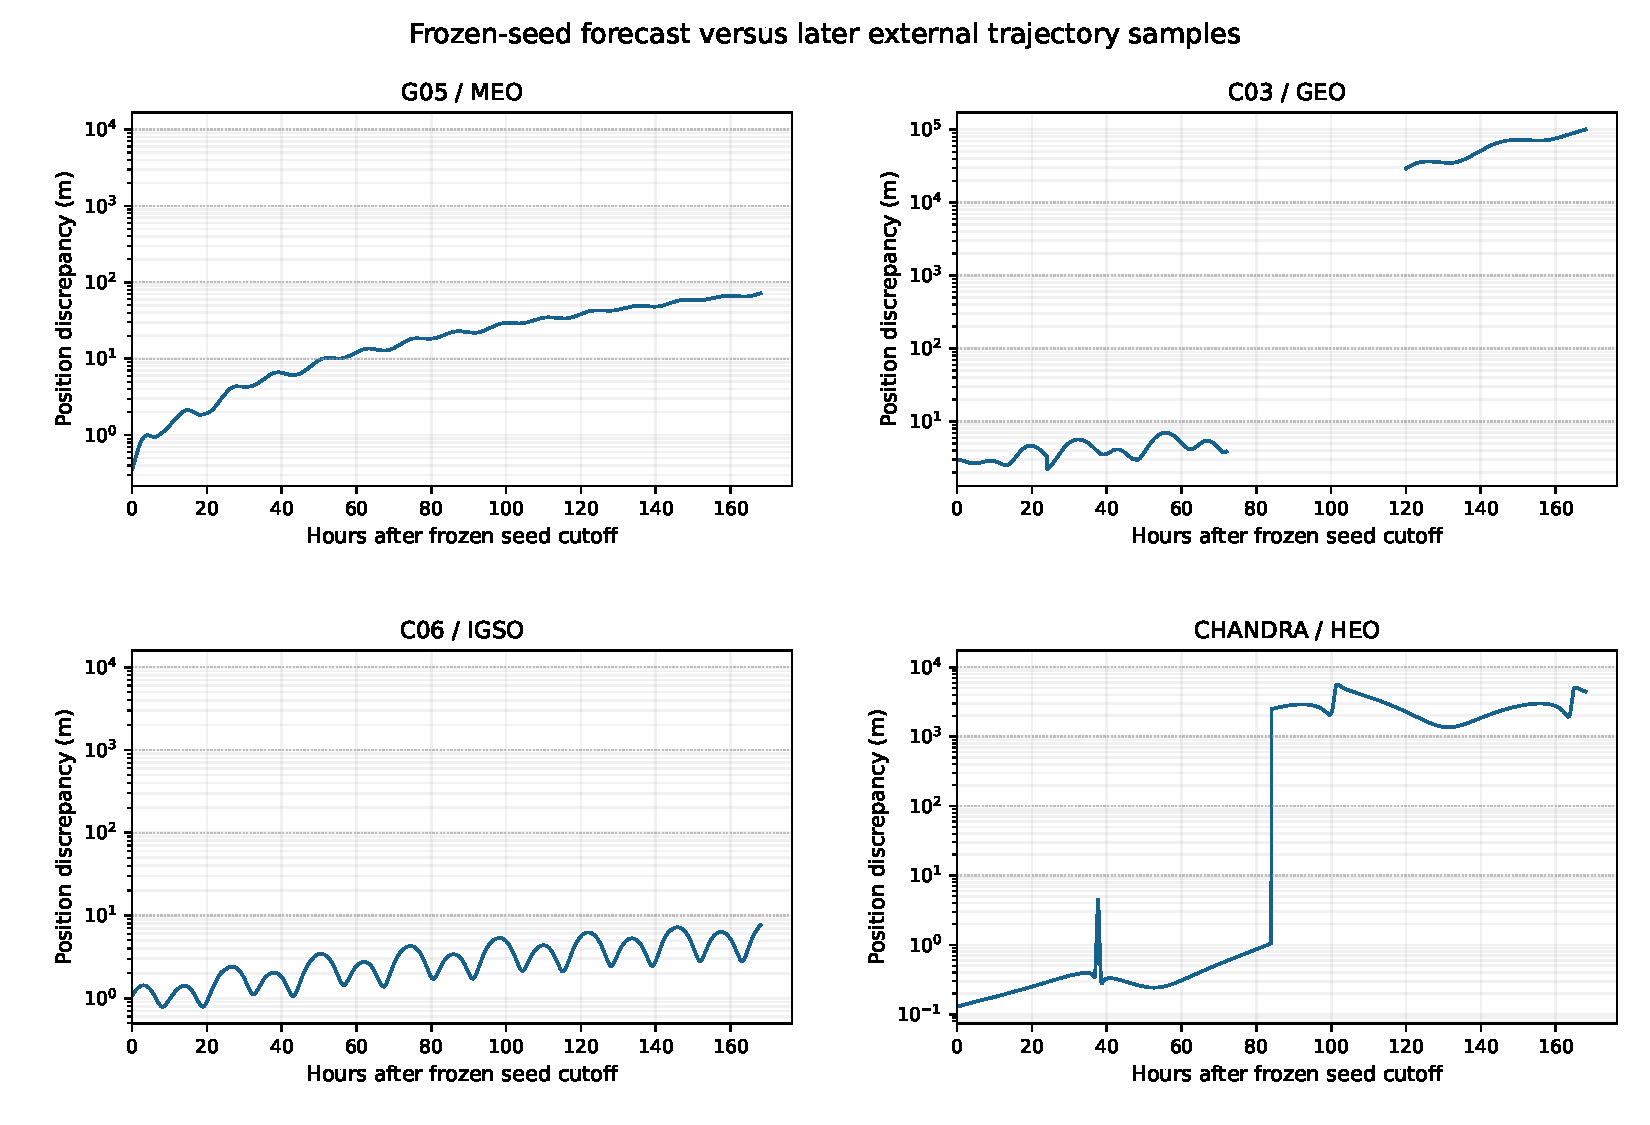
\includegraphics[width=\linewidth]{../results/orbit_accuracy_confirmation_cpu_verified/forecast_error_curves.pdf}
\end{center}
The selection rule was frozen before this date's errors were evaluated. The
C03 reference gap is blank; connecting its endpoints would imply unavailable
measurements. Chandra's source discontinuity is retained. Lines join only
available adjacent samples and do not certify error between samples or beyond
the declared window.

\clearpage
